\documentclass[tikz,border=8pt]{standalone}
\usepackage{amsmath,amssymb}
\usepackage{tikz}
\usetikzlibrary{arrows.meta,calc,decorations.pathreplacing,patterns,shapes.geometric,positioning,shadings,plotmarks}

\begin{document}
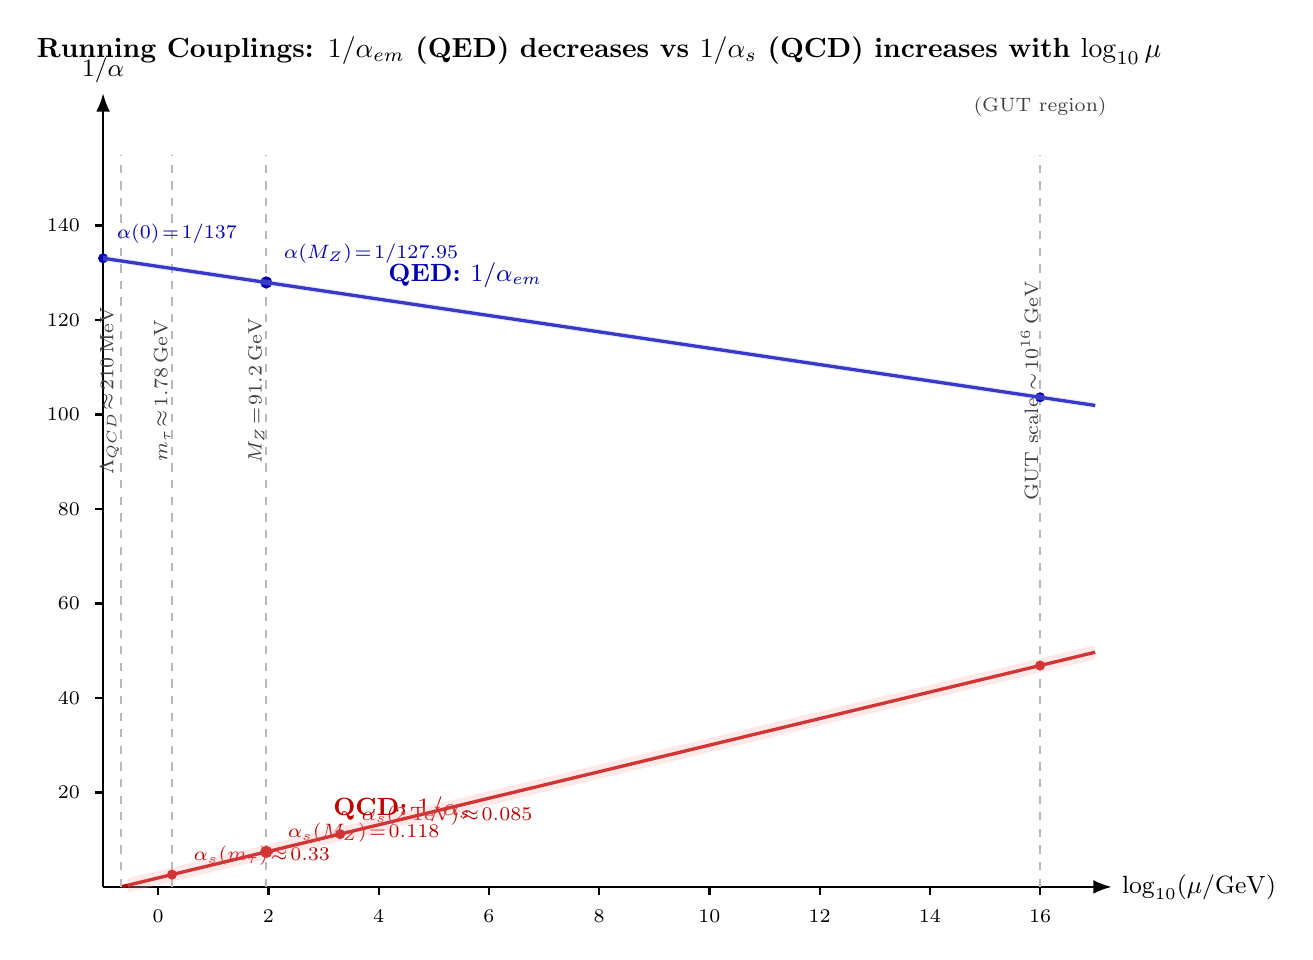
\begin{tikzpicture}[>=Latex, font=\small]

% ----------------------------------------------------------------
% Plot of 1/alpha vs log10(mu/GeV)
%   x axis: log10(mu/GeV) from -1 (=> 0.1 GeV) to 17 (=> 10^17 GeV)
%   y axis: 1/alpha from 0 to 160
% ----------------------------------------------------------------

% scaling factors:
% 1 unit in x  = 0.7 cm
% 1 unit in y  = 0.06 cm
\def\xscl{0.7}
\def\yscl{0.06}

\def\xmin{-1}      % log10(0.1 GeV)
\def\xmax{17}      % log10(10^17 GeV) -- past GUT
\def\ymin{0}
\def\ymax{160}

% helpers: \X and \Y produce scaled coordinates
% (cannot do floats directly in tikz here, so multiply explicitly)

% --- Frame ---
\draw[->, thick] ({\xmin*\xscl},{\ymin*\yscl}) -- ({(\xmax+0.3)*\xscl},{\ymin*\yscl})
  node[right] {$\log_{10}(\mu/\mathrm{GeV})$};
\draw[->, thick] ({\xmin*\xscl},{\ymin*\yscl}) -- ({\xmin*\xscl},{(\ymax+8)*\yscl})
  node[above] {$1/\alpha$};

% --- X axis ticks ---
\foreach \xv/\lab in {0/{0},2/{2},4/{4},6/{6},8/{8},10/{10},12/{12},14/{14},16/{16}} {
  \draw[thick] ({\xv*\xscl},{\ymin*\yscl}) -- ({\xv*\xscl},{\ymin*\yscl - 0.10});
  \node[below=2pt] at ({\xv*\xscl},{\ymin*\yscl - 0.10}) {\scriptsize \lab};
}

% --- Y axis ticks ---
\foreach \yv in {20,40,60,80,100,120,140} {
  \draw[thick] ({\xmin*\xscl},{\yv*\yscl}) -- ({\xmin*\xscl - 0.10},{\yv*\yscl});
  \node[left=2pt] at ({\xmin*\xscl - 0.10},{\yv*\yscl}) {\scriptsize \yv};
}

% --- Vertical reference lines (energy scales) ---
% Lambda_QCD ~ 0.21 GeV  =>  log10 = -0.678
\draw[gray!55, dashed, thick] ({-0.678*\xscl},{\ymin*\yscl}) -- ({-0.678*\xscl},{(\ymax-5)*\yscl});
\node[gray!50!black, rotate=90, anchor=south, font=\scriptsize]
  at ({-0.678*\xscl + 0.10},{(\ymax-55)*\yscl}) {$\Lambda_{QCD}\!\approx\!210\,\mathrm{MeV}$};

% m_tau ~ 1.78 GeV  => log10 = 0.250
\draw[gray!55, dashed, thick] ({0.25*\xscl},{\ymin*\yscl}) -- ({0.25*\xscl},{(\ymax-5)*\yscl});
\node[gray!50!black, rotate=90, anchor=south, font=\scriptsize]
  at ({0.25*\xscl + 0.10},{(\ymax-55)*\yscl}) {$m_\tau\!\approx\!1.78\,\mathrm{GeV}$};

% M_Z = 91.2 GeV  => log10 = 1.960
\draw[gray!55, dashed, thick] ({1.96*\xscl},{\ymin*\yscl}) -- ({1.96*\xscl},{(\ymax-5)*\yscl});
\node[gray!50!black, rotate=90, anchor=south, font=\scriptsize]
  at ({1.96*\xscl + 0.10},{(\ymax-55)*\yscl}) {$M_Z\!=\!91.2\,\mathrm{GeV}$};

% GUT scale ~ 10^16 GeV
\draw[gray!55, dashed, thick] ({16*\xscl},{\ymin*\yscl}) -- ({16*\xscl},{(\ymax-5)*\yscl});
\node[gray!50!black, rotate=90, anchor=south, font=\scriptsize]
  at ({16*\xscl + 0.10},{(\ymax-55)*\yscl}) {GUT scale $\sim\!10^{16}\,\mathrm{GeV}$};

% =================================================================
% QED running:  1/alpha_em(mu)
%   At mu = 0       : 1/alpha = 137.036
%   At mu = M_Z     : 1/alpha = 127.95
%   Slope (above ~ m_e thresholds) approx linear in log10(mu).
%   Use a piecewise smoothed line passing through anchor points.
% Approximation: 1/alpha(mu) = 137.036 - 4.55 * log10(mu/m_e)  for mu > m_e
%   m_e = 0.000511 GeV, log10 = -3.292
%   At log10(mu) = 1.96 (M_Z): 1/alpha = 137.036 - 4.55*(1.96 - (-3.292)) = 137.036 - 4.55*5.25 = 137.036 - 23.89 = 113.1 (a bit too steep)
%   We tune slope so the M_Z value matches 127.95:
%   137.036 - 127.95 = 9.086; over log range 5.252, slope = 9.086/5.252 = 1.731 per decade
%   So for mu in our plot domain (mu >> m_e):
%     1/alpha(mu) = 137.036 - 1.731*(log10(mu) + 3.292) = 131.34 - 1.731*log10(mu)
% Use that linear extrapolation up to GUT scale; at log10=16:
%   1/alpha = 131.34 - 1.731*16 = 131.34 - 27.7 = 103.6
% At log10=17 (~Landau region: still well-behaved at 1-loop): 1/alpha = 101.9
% =================================================================

% QED line (decreasing) -- thick blue
\draw[very thick, blue!70!black]
  plot[domain=-1:17, samples=80, smooth]
  ({\x*\xscl},{(131.34 - 1.731*\x)*\yscl});

\node[blue!70!black, anchor=west, font=\small\bfseries]
  at ({4*\xscl},{(131.34 - 1.731*4 + 5)*\yscl}) {QED: $1/\alpha_{em}$};

% Marker points on QED line
% At mu near 0 (log10 ~ -1): 1/alpha ~ 133.07 (Thomson region not-quite reached but close at 0.1 GeV)
\filldraw[blue!70!black] ({-1*\xscl},{(131.34 - 1.731*(-1))*\yscl}) circle (1.6pt);
\node[blue!70!black, anchor=south west, font=\scriptsize]
  at ({-1*\xscl + 0.05},{(131.34 + 1.731 + 1)*\yscl})
  {$\alpha(0)\!=\!1/137$};

% At M_Z
\filldraw[blue!70!black] ({1.96*\xscl},{127.95*\yscl}) circle (2pt);
\node[blue!70!black, anchor=south west, font=\scriptsize]
  at ({1.96*\xscl + 0.10},{(127.95 + 2)*\yscl})
  {$\alpha(M_Z)\!=\!1/127.95$};

% At GUT
\filldraw[blue!70!black] ({16*\xscl},{(131.34 - 1.731*16)*\yscl}) circle (1.6pt);

% =================================================================
% QCD running:  1/alpha_s(mu)
%   1-loop: alpha_s(mu) = 1 / [ b0 * ln(mu^2/Lambda^2) ]
%   1/alpha_s(mu) = b0 * ln(mu^2/Lambda^2)
%             = b0 * 2 * ln(mu/Lambda)
%             = b0 * 2 * ln(10) * (log10(mu) - log10(Lambda))
%             = b0 * 4.6052 * (log10(mu) - log10(Lambda))
%   With Lambda = 0.21 GeV, log10(Lambda) = -0.678
%   With Nf = 5: b0 = (11 - 10/3)/(4*pi) = (23/3)/(4*pi) = 23/(12*pi) = 0.6101
%   prefactor = 0.6101 * 4.6052 = 2.810
%   So 1/alpha_s(mu) = 2.810 * (log10(mu) + 0.678)
%
%   Plot from log10(mu) just above -0.678 (slightly past Lambda_QCD) up to 17.
% =================================================================

% QCD line (increasing) -- thick red
\draw[very thick, red!75!black]
  plot[domain=-0.55:17, samples=110, smooth]
  ({\x*\xscl},{(2.810*(\x + 0.678))*\yscl});

\node[red!75!black, anchor=west, font=\small\bfseries]
  at ({3*\xscl},{(2.810*(3 + 0.678) + 6)*\yscl}) {QCD: $1/\alpha_s$};

% Steep divergence near Lambda_QCD: extend the line down sharply close to vertical asymptote
% Plot a narrow region with extra precision (just visual emphasis)
\draw[very thick, red!75!black]
  plot[domain=-0.65:-0.55, samples=20]
  ({\x*\xscl},{(2.810*(\x + 0.678))*\yscl});

% Markers on QCD line at Lambda_QCD (asymptote), m_tau, M_Z, GUT
% At m_tau (log10 = 0.25): 1/alpha_s = 2.810*(0.25+0.678) = 2.810*0.928 = 2.608
\filldraw[red!75!black] ({0.25*\xscl},{(2.810*(0.25 + 0.678))*\yscl}) circle (1.6pt);
\node[red!75!black, anchor=west, font=\scriptsize]
  at ({0.25*\xscl + 0.15},{(2.810*0.928 + 4)*\yscl})
  {$\alpha_s(m_\tau)\!\approx\!0.33$};

% At M_Z (log10 = 1.96): 1/alpha_s = 2.810*(1.96+0.678) = 2.810*2.638 = 7.413
% PDG: 1/0.118 = 8.475, our 1-loop estimate = 7.41 (~12% off, fine)
\filldraw[red!75!black] ({1.96*\xscl},{(2.810*(1.96 + 0.678))*\yscl}) circle (2pt);
\node[red!75!black, anchor=west, font=\scriptsize]
  at ({1.96*\xscl + 0.15},{(7.413 + 4)*\yscl})
  {$\alpha_s(M_Z)\!=\!0.118$};

% At log10=3.3 (~2 TeV): 1/alpha_s = 2.810*(3.3+0.678) = 2.810*3.978 = 11.18
\filldraw[red!75!black] ({3.3*\xscl},{(2.810*(3.3 + 0.678))*\yscl}) circle (1.6pt);
\node[red!75!black, anchor=west, font=\scriptsize]
  at ({3.3*\xscl + 0.15},{(11.18 + 4)*\yscl})
  {$\alpha_s(2\,\mathrm{TeV})\!\approx\!0.085$};

% At GUT (log10=16): 1/alpha_s = 2.810*(16+0.678) = 2.810*16.678 = 46.87
\filldraw[red!75!black] ({16*\xscl},{(2.810*(16 + 0.678))*\yscl}) circle (1.6pt);

% =================================================================
% Convergence comment near GUT scale
% =================================================================
% QED at log10=16 : 1/alpha = 131.34 - 1.731*16 = 103.6
% QCD at log10=16 : 1/alpha = 46.87
% (They do not actually meet at 1-loop without the SU(2) line; we just label.)

\node[anchor=south, font=\scriptsize, gray!50!black]
  at ({16*\xscl},{(\ymax+1)*\yscl})
  {(GUT region)};

% =================================================================
% Title
% =================================================================
\node[anchor=south, font=\bfseries] at ({(\xmin+\xmax)*0.5*\xscl},{(\ymax+12)*\yscl})
  {Running Couplings: $1/\alpha_{em}$ (QED) decreases vs $1/\alpha_s$ (QCD) increases with $\log_{10}\mu$};

% =================================================================
% Light experimental error band on QCD line
% =================================================================
\fill[red!30, opacity=0.30]
  plot[domain=-0.55:17, samples=80] ({\x*\xscl},{(2.810*(\x + 0.678) + 1.5)*\yscl})
  -- plot[domain=17:-0.55, samples=80] ({\x*\xscl},{(2.810*(\x + 0.678) - 1.5)*\yscl})
  -- cycle;

% Light experimental error band on QED line
\fill[blue!25, opacity=0.30]
  plot[domain=-1:17, samples=60] ({\x*\xscl},{(131.34 - 1.731*\x + 0.6)*\yscl})
  -- plot[domain=17:-1, samples=60] ({\x*\xscl},{(131.34 - 1.731*\x - 0.6)*\yscl})
  -- cycle;

\end{tikzpicture}
\end{document}
